\documentclass[11pt]{article}

\usepackage[letterpaper,margin=1in]{geometry}
\usepackage[T1]{fontenc}
\usepackage{lmodern}
\usepackage{microtype}
\usepackage{amsmath,amssymb}
\usepackage{array}
\usepackage{booktabs}
\usepackage{graphicx}
\usepackage{caption}
\usepackage{enumitem}
\usepackage{float}
\usepackage{tabularx}
\usepackage[numbers,sort&compress]{natbib}
\usepackage{xcolor}
\usepackage{hyperref}
\hypersetup{
  colorlinks=true,
  citecolor=blue!55!black,
  linkcolor=blue!45!black,
  urlcolor=blue!55!black
}
\setlist{nosep,leftmargin=*}
\captionsetup{font=small,labelfont=bf}
\renewcommand{\thepart}{\Roman{part}}
\renewcommand{\thesection}{\thepart.\arabic{section}}
\renewcommand{\thesubsection}{\thesection.\arabic{subsection}}
\renewcommand{\theHsection}{\thepart.\arabic{section}}
\renewcommand{\theHsubsection}{\theHsection.\arabic{subsection}}
\newcolumntype{Y}{>{\raggedright\arraybackslash}X}

\title{\bfseries Importance Weighted Autoencoders on Dynamically Binarized
MNIST: Reproduction and Extension}
\author{
Gil Chen -- 316019975\\
Guy Raz -- 302632740\\[0.4em]
\small Deep Generative Models of Texts and Images
}
\date{18 July 2026}

\begin{document}
\maketitle

\part{Reproduction of Importance Weighted Autoencoders}

\begin{center}
\begin{minipage}{0.88\textwidth}
\begin{center}
\textbf{\large Abstract}
\end{center}
This part documents a compute-conscious reproduction of the
one-stochastic-layer Importance Weighted Autoencoder (IWAE) experiment of
\citet{burda2016importance}.  The reconstruction preserves the paper's
generative model, recognition model, objective with 50 importance samples,
dynamic MNIST training binarization, initialization, optimizer, and staged
learning-rate schedule, while using a modern PyTorch and PyTorch Lightning
implementation.  After 121 training passes on an Apple M1 GPU, the model
obtains a 5,000-sample test negative log-likelihood estimate of 87.804 nats and
25 active latent units.  The latter matches the paper's reported value,
whereas the likelihood remains 3.024 nats above its 84.78-nat result.  This gap
is interpreted in light of the present run using only 3.7\% of the paper's
3,280-pass optimization budget.  The result establishes a documented,
reproducible IWAE baseline without claiming full numerical replication.
\end{minipage}
\end{center}

\section{Introduction}
Variational autoencoders (VAEs) combine amortized inference with
reparameterized stochastic optimization
\citep{kingma2014auto,rezende2014stochastic}.  Their standard evidence lower
bound (ELBO), however, may provide a weak training signal when the approximate
posterior is restrictive.  IWAE replaces the single-sample ELBO with an
importance-weighted bound and empirically learns representations with more
active latent variables \citep{burda2016importance}.

The objective of this reproduction is not to maximize MNIST performance at
arbitrary computational cost.  It is to establish a traceable result that
(i) remains close enough to the original experiment for an academically
meaningful comparison, (ii) runs on a 16\,GB Apple M1 or a modest Colab
accelerator, and (iii) clearly separates faithful scientific choices from
implementation-level modernization.

\section{Importance-weighted variational inference}
For observation $x$, latent variable $z$, generative model
$p_\theta(x,z)$, and recognition model $q_\phi(z\mid x)$, draw
$z_{1:K}\stackrel{\mathrm{iid}}{\sim}q_\phi(z\mid x)$ and define
\begin{equation}
 w_k = \frac{p_\theta(x,z_k)}{q_\phi(z_k\mid x)}.
\end{equation}
The IWAE objective is
\begin{equation}
 \mathcal{L}_K(x)
 = \mathbb{E}_{z_{1:K}}\!
   \left[\log\left(\frac{1}{K}\sum_{k=1}^{K}w_k\right)\right].
 \label{eq:iwae}
\end{equation}
Under the conditions given by \citet{burda2016importance},
$\mathcal{L}_1\leq\mathcal{L}_K\leq\log p_\theta(x)$ and the expected bound
is nondecreasing in $K$.  Thus $K>1$ gives a tighter variational objective,
although a tighter bound does not by itself guarantee a better finite-budget
optimizer trajectory.  We minimize the corresponding negative bound in nats.

\section{Reconstruction design}
\subsection{Data protocol}
The paper describes the standard 60,000/10,000 MNIST train/test split; the
released code reserves 400 of the 60,000 training examples for validation
\citep{burda2016importance,burda2015code}.  We follow that implementation-level
59,600/400/10,000 split.  Each training image is converted to a Bernoulli
sample on every retrieval, following the random-binarization protocol in the
authors' implementation.  Validation and test examples instead receive one
seeded Bernoulli draw that remains fixed.  This documented deviation reduces
evaluation noise and makes repeated evaluations use identical observations,
but it prevents a perfectly like-for-like comparison with every stochastic
evaluation detail of the original code.

\subsection{Architecture and initialization}
Table~\ref{tab:architecture} gives the complete architecture.  Both networks
are multilayer perceptrons with two 200-unit $\tanh$ hidden layers.  The
recognition network outputs the mean and log standard deviation of a
50-dimensional diagonal Gaussian.  The decoder outputs 784 Bernoulli logits.
Weights use Glorot uniform initialization and biases are initially zero,
matching the original source \citep{glorot2010understanding,burda2015code}.
The decoder's output bias is then set to the empirical training-pixel log odds,
as in the source experiment.  This initialization is explicit because
PyTorch's default \texttt{Linear} initialization is not Glorot uniform;
explicitness here is experimental fidelity rather than redundant framework
code.

\begin{table}[H]
\centering
\caption{One-stochastic-layer IWAE architecture.  The stochastic layer is the
50-dimensional latent variable; each network also contains two deterministic
hidden layers.}
\label{tab:architecture}
\begin{tabular}{ll}
\toprule
Component & Specification \\
\midrule
Input & $x\in\{0,1\}^{784}$ \\
Encoder & $784\rightarrow200\rightarrow200\rightarrow(50+50)$ \\
Approximate posterior & diagonal Gaussian \\
Decoder & $50\rightarrow200\rightarrow200\rightarrow784$ \\
Likelihood & factorized Bernoulli \\
Activation & $\tanh$ \\
Parameters & 425,284 \\
Training particles & $K=50$ \\
\bottomrule
\end{tabular}
\end{table}

\subsection{Optimization and reproducibility}
\begin{table}[H]
\centering
\caption{Optimization, software, and hardware configuration for the completed
IWAE run.}
\label{tab:setup}
\begin{tabularx}{\textwidth}{@{}>{\raggedright\arraybackslash\bfseries}p{0.25\textwidth}Y@{}}
\toprule
Setting & Value \\
\midrule
Optimizer & Adam \citep{kingma2015adam} \\
Initial learning rate & $10^{-3}$ \\
Adam parameters & $(\beta_1,\beta_2)=(0.9,0.999)$ and
  $\epsilon=10^{-4}$ \\
Batch size & 20 \\
Numeric precision & 32-bit floating point \\
Learning-rate schedule & Multiply by $\gamma=10^{-1/7}$ at cumulative passes
  $\{1,4,13,40,121,364,1093,3280\}$ \\
Scheduler implementation & PyTorch \texttt{MultiStepLR}; the completed
  checkpoint used an algebraically equivalent direct schedule whose logged
  rates match the paper \\
Global random seed & 236 \\
Software & PyTorch 2.13.0; Lightning 2.6.5; torchvision 0.28.0;
  TorchMetrics 1.9.0 \\
Host system & macOS 15.7.7; Apple M1; 16\,GB unified memory \\
Accelerator & Metal Performance Shaders (MPS) \\
Persisted artifacts & Checkpoints, hyperparameters, and per-epoch metrics \\
\bottomrule
\end{tabularx}
\end{table}

\section{Evaluation protocol}
Test negative log likelihood (NLL) is estimated with
$-\mathcal{L}_{5000}$, evaluated in chunks of 100 particles to bound device
memory.  Chunking accumulates the same log-sum-exp as an unchunked estimate and
therefore changes memory use, not the estimator.  Lower NLL is better.

Following \citet{burda2016importance}, latent dimension $j$ is counted as
active when
\begin{equation}
 \operatorname{Var}_{x}\!
 \left[\mathbb{E}_{q_\phi(z\mid x)}[z_j]\right] > 0.01.
\end{equation}
This diagnostic measures variation in posterior means across the data; it is
not proof that every active coordinate is semantically disentangled.

\section{Results}
\begin{table}[H]
\centering
\caption{Published target and completed reproduction.  NLL values are in
nats.  The training and validation quantities are $-\mathcal{L}_{50}$ and
must not be compared numerically with test $-\mathcal{L}_{5000}$.}
\label{tab:results}
\begin{tabular}{lrr}
\toprule
Quantity & Paper & This run \\
\midrule
Training passes & 3,280 & 121 \\
Train $-\mathcal{L}_{50}$ & -- & 90.268 \\
Validation $-\mathcal{L}_{50}$ & -- & 90.400 \\
Test $-\mathcal{L}_{5000}$ & 84.78 & 87.804 \\
Active units & 25 & 25 \\
Wall-clock time & -- & 74.2 min \\
\bottomrule
\end{tabular}
\end{table}

The optimization curves in Figure~\ref{fig:curve} fall rapidly and remain
close after the early passes.  Both recorded minima occur at pass 121.  This
supports checkpoint selection at the end of the available budget, but it does
not establish convergence: the original schedule allocates another 3,159
passes.

\begin{figure}[htbp]
\centering
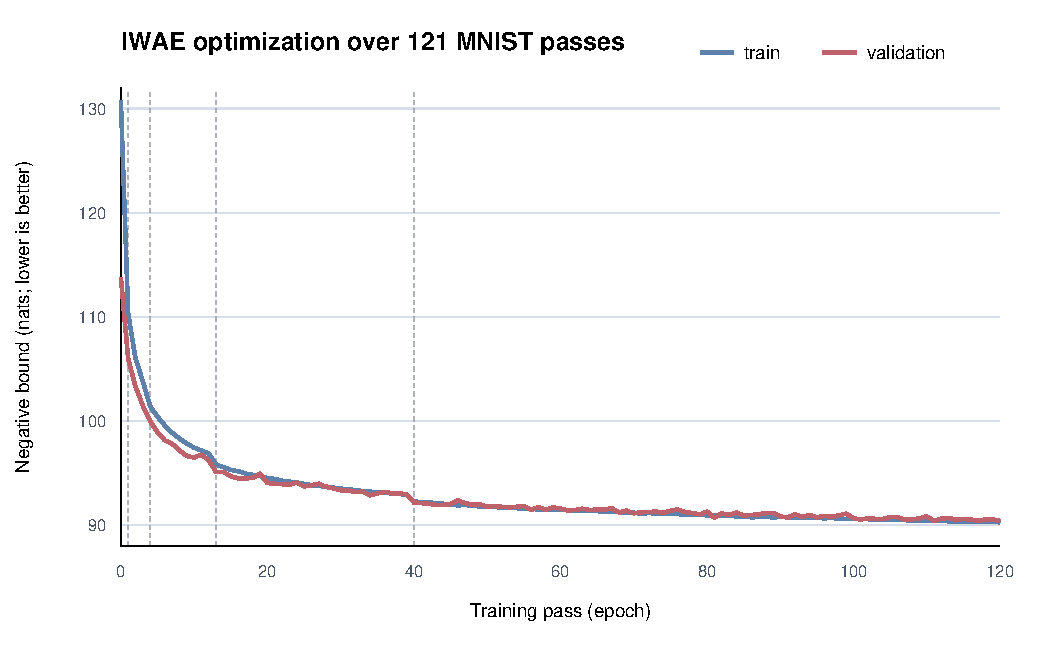
\includegraphics[width=0.88\textwidth]{figures/iwae_learning_curve.pdf}
\caption{Epoch-level negative IWAE bounds for the completed 121-pass run.
Dashed vertical lines denote learning-rate milestones within the observed
window.  Lower is better.}
\label{fig:curve}
\end{figure}

The 3.024-nat gap from the published test NLL is unsurprising under the
truncated budget.  The run consumes only $121/3280=3.69\%$ of the paper's
training passes.  Differences in the fixed evaluation draw, random-number
generators, floating-point kernels, and framework implementation are secondary
possible contributors.  Because these factors are not independently ablated,
the optimization budget is the strongest explanation, not a formally isolated
cause.

The prior samples in Figure~\ref{fig:samples} are recognizably digit-like and
cover several digit classes.  Some strokes remain ambiguous or fragmented.
This is useful qualitative evidence that the decoder learned the data domain,
but sample inspection is not substituted for likelihood-based comparison.

\begin{figure}[htbp]
\centering
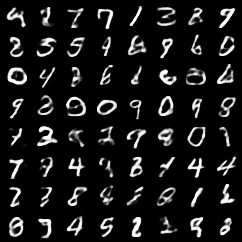
\includegraphics[width=0.42\textwidth]{figures/iwae_samples_epoch120.png}
\caption{An $8\times8$ grid of prior predictive decoder probabilities from
epoch index 120 (after 121 training passes).  Brightness represents Bernoulli
mean rather than a thresholded pixel draw.}
\label{fig:samples}
\end{figure}

\section{Faithfulness and implementation modernization}
The scientific core is preserved: random-binarized training data,
architecture, latent size, $K=50$ objective, initialization, optimizer
hyperparameters, and milestone schedule.  Device transfer, optimizer stepping,
checkpoint serialization, metrics, and distributed-safe logging use maintained
framework abstractions.  Replacing those mechanics with handwritten
equivalents would increase maintenance surface without increasing fidelity.

Three choices are intentionally modern.  First, evaluation binarization is
fixed per example for repeatability.  Second, a chunked 5,000-particle
calculation makes evaluation feasible on 16\,GB unified memory.  Third, the
executable interface and saved configuration make every run self-describing.
Only the first changes the stochastic evaluation protocol; the latter two are
implementation-level changes.

\section{Limitations}
This is a single-seed, truncated-budget reproduction.  Consequently it cannot
estimate run-to-run uncertainty or claim numerical replication of the
published NLL.  MNIST likelihood also says little about behavior on natural
images or text.  The 74.2-minute duration is reconstructed from artifact
timestamps rather than a trainer-emitted duration field, so it should be read
as elapsed wall-clock time to timestamp precision.  Finally, the active-unit
threshold is inherited from the source study and is only one representation
diagnostic.

\section{Conclusion}
The completed baseline demonstrates that the central one-stochastic-layer,
50-particle IWAE experiment is practical on an M1-class device.  It reproduces
the published active-unit count and produces coherent samples, while its
likelihood gap is consistent with a deliberately much shorter training budget.
The resulting checkpoint, metrics, and documented deviations form a credible
and reproducible reconstruction of the selected paper condition.

\section*{Artifact availability}
The run can be reproduced from the project root with:
\begin{quote}\small\ttfamily
uv run iwae train iwae --accelerator mps --max-epochs 121
\end{quote}
The archived checkpoint is
\path{outputs/iwae/checkpoints/epoch-0120.ckpt}; the test protocol uses:
\begin{quote}\small\ttfamily
uv run iwae evaluate outputs/iwae/checkpoints/epoch-0120.ckpt
--accelerator mps
\end{quote}

\clearpage
\setcounter{section}{0}
\part{Doubly Reparameterized Gradient Study}

\begin{center}
\begin{minipage}{0.88\textwidth}
\begin{center}
\textbf{\large Abstract}
\end{center}
This part evaluates the doubly reparameterized gradient (DReG) estimator of
\citet{tucker2019doubly} as a controlled extension of the completed IWAE
baseline.  The data, architecture, initialization, generative objective,
optimizer, particle count, training budget, and evaluation procedure are held
fixed while the inference-network gradient estimator is changed.  At the
matched 121-pass budget, DReG obtains a test NLL of 87.480 nats and 26 active
units, compared with 87.804 nats and 25 active units for IWAE.  The 0.323-nat
NLL reduction is a modest numerical improvement, but a single paired seed does
not establish a reliable population-level advantage.
\end{minipage}
\end{center}

\section{Motivation and hypothesis}
As the number of importance samples grows, the conventional inference-network
gradient estimator can suffer a deteriorating signal-to-noise ratio.  DReG
removes a high-variance score-function component by applying
reparameterization a second time \citep{tucker2019doubly}.  The working
hypothesis is that, under an otherwise identical $K=50$ experiment, this
estimator will improve inference-network optimization without changing the
model or generative objective.

\section{Controlled experimental design}
The comparison holds fixed the MNIST split and binarization draws, network
architecture, initialization seed, $K=50$, optimizer settings, learning-rate
schedule, training budget, and evaluation implementation.  The intended
independent variable is the inference-network gradient estimator.  Both
conditions use seed 236 and 121 training passes, and each test result is
computed from the checkpoint selected by validation NLL.

The primary comparison is test NLL estimated with
$-\mathcal{L}_{5000}$.  Active units will remain a secondary representation
diagnostic.  Kernel Inception Distance (KID)
\citep{binkowski2018demystifying}, computed in the fixed MNIST-classifier
feature space, will provide a course-specific sample diagnostic.  KID was not
reported by the original IWAE paper and is comparable only when the feature
extractor, real observations, subset configuration, sample count, and seed are
identical.

\section{Results}
\begin{table}[H]
\centering
\caption{Matched single-seed comparison after 121 training passes.  Lower NLL
is better.  Active units are descriptive rather than an ordered quality
metric.}
\label{tab:dreg-results}
\begin{tabular}{lrr}
\toprule
Metric & IWAE & IWAE-DReG \\
\midrule
Training passes & 121 & 121 \\
Selected checkpoint epoch & 120 & 114 \\
Train $-\mathcal{L}_{50}$ at selected epoch & 90.268 & 89.652 \\
Validation $-\mathcal{L}_{50}$ at selected epoch & 90.400 & 89.661 \\
Test $-\mathcal{L}_{5000}$ & 87.804 & \textbf{87.480} \\
Active units & 25 & 26 \\
Active training time (min) & 74.2 & approximately 71.5 \\
KID & not measured & not measured \\
\bottomrule
\end{tabular}
\end{table}

Relative to IWAE, DReG reduces the estimated test NLL by 0.323 nats
(approximately 0.37\%) and increases the active-unit count by one.  The DReG
checkpoint was selected at epoch 114, where its validation bound was 0.739
nats lower than the IWAE checkpoint's validation bound.  Both models were
nevertheless allowed the same 121-pass training budget.

\section{Discussion}
The result is directionally favorable to DReG, but the effect is small relative
to the remaining gap from the paper's 84.78-nat result.  It is therefore more
accurate to report a modest single-seed improvement than either a clear
estimator win or no improvement.  The active-unit change from 25 to 26 is also
too small to support a strong representation claim.

The interrupted training sessions make the reported active training time an
artifact-timestamp estimate, although it remains similar to the IWAE runtime.
KID was not measured, so the likelihood result cannot be extended to a claim
about sample quality.  Matched repetitions with seeds 237 and 238 are needed
to estimate variability and determine whether the NLL difference is
consistent rather than seed-specific.

\section{Conclusion}
Under the completed seed-236 comparison, DReG improves test NLL from 87.804 to
87.480 nats while using one additional active latent unit and comparable
training time.  This is a measurable but modest improvement.  Without
replicated seeds or a sample-quality metric, the evidence does not justify a
broad claim that DReG is reliably superior; it supports only a limited
within-seed advantage under the present compute budget.

\clearpage
\bibliographystyle{plainnat}
\bibliography{references}

\end{document}
